\documentclass[12pt,fleqn]{article}\usepackage{../../common}
\begin{document}
Gazlar, Sıvılar - 3

Taşınımsal Nakil (Convective Transport)

Bu kavramı anlamak için bir akışın önünde duran geçirgen bir yüzey
düşünelim. Akışı temsil eden hız alanını biliyoruz, bu alanın yüzeydeki
vektörleri bir sıvı parçacığının o noktadaki, o andaki hareketini gösteriyor.

Bir sıvı parçacığı yeri değiştirilebilecek belli oranda bir madde, öğe
içerebilir, ve o parçacık yüzeyin bir tarafından diğer tarafına geçtiğinde
parçacıkla beraber ögenin yeri de değişmiş olur. Dikkat nakletme direk bir
geçiş ima eder, hızın normal bileşenine oranla bir geçiştir bu. Bu bağlamda
hızın sadece normal (yüzeye dik) olan bileşenine bakarız, çünkü yüzeye
teğet olan bileşen hiç bir geçiş oluşturmazdı, yüzeye paralel olan bir
gidiştir bu. Tabii ki yüzeyin farklı noktalarında farklı hızlar, ve farklı
öğe değerleri olabilir, bu sebeple taşınımsal naklinin matematiksel
tarifi bu farklılıkları göz önüne almalıdır. 

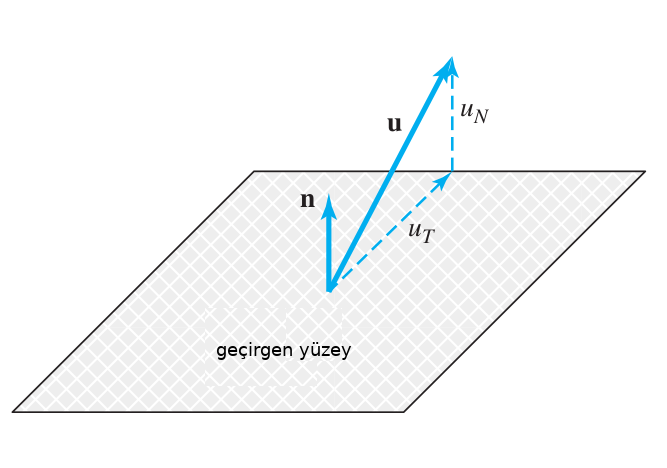
\includegraphics[width=20em]{phy_030_fluid2_04.png}

Şimdi taşınımsal nakil $\Gamma_C$ ile tanımlarsak, bu değişken bir zaman anında
sıvının akışı sebebiyle bir öğenin yüzeyi geçme oranı olacaktır. Eğer $\epsilon$
birim kütledeki öğe miktarı ise, $\rho \epsilon$ birim hacimdeki o öğenin
miktarı olur (çünkü $\rho$ yoğunluk, birim hacimdeki kütle). O zaman herhangi
bir noktada bu ögenin hız alanı içinde yerel bir hız vektörü yönünde anlık
taşınma oranı / hızı $\rho \epsilon u$ olur, $u = \bar{u}(\bar{x},t)$. Bu
oranı yüzeyden geçise tercüme edersek, yüzeydeki $n$ normaline sahip $\ud S$
yüzey alanından geçiş oranı

$$
\delta \Gamma_C = \rho \epsilon (u \cdot n) \ud S
$$

Daha önce belirttik yüzeyin her noktasında farklı nakil oranları olabilir,
tüm geçirgen yüzey için $\Gamma_C$ hesabı için her yüzey ögesinden olan geçiş
oranlarını bir yüzey entegrali ile toplarız,

$$
\Gamma_C = \int_S \rho \epsilon (u \cdot n) \ud S
$$

Bu tür entegrallere taşınımsal akış entegrali (convective flux integral) ya da
kısaca taşınımsal entegral ismi veriliyor. Fakat dikkat bu hesabın sonucu bir
oran (birim zamandaki öğe), akış değil (birim alandaki öğenin birim zamandaki
hızı).

Kabaca öğe dedik, ama pek çok kavram üstteki formüller kapsamına giriyor, mesela
kütle hesabı için $\epsilon = 1$ diyebiliriz, ya da momentum için
$\epsilon = u$. Isı taşınımı da benzer şekilde temsil edilir.

Reynolds Nakletme Teorisi (Reynold's Transport Theorem)

Daha önce pür kütle hesabında $\epsilon = 1$ üzerinden türetilen muhafaza
kanununu görmüştük,

$$
\frac{\partial \rho}{\partial t} + \nabla \cdot (\rho u ) = 0
$$

Ya da 

$$
\frac{\partial \rho}{\partial t} + \bdiv (\rho u ) = 0
\mlabel{1}
$$

Bu $\epsilon = 1$ durumudur, daha genel $\epsilon$ için

$$
\frac{\partial \rho \epsilon}{\partial t} + \bdiv (\rho \epsilon u ) = 0
$$

elde edileceğini ispat etmek zor değil. Terim $\bdiv$ içindekilere çarpım
kuralını uygularsak, ve $\epsilon$ yerine $\phi$ kullanınca açılım [3, sf. 24]

$$
\rho \frac{\partial \phi}{\partial t} +
\phi \frac{\partial \rho}{\partial t} + 
\rho \bdiv (\phi u ) +
\phi \bdiv (\rho u ) = 0
$$

$$
\rho \frac{\partial \phi}{\partial t} +
\phi \bdiv (\rho u ) +
\phi \left(
  \frac{\partial \phi}{\partial t} + \bdiv (\rho u ) 
\right) = 0
$$

Akış alanı süreklilik kuralını destekliyor, yani (1) geçerli, o zaman
parantez içindekiler yok sayılır,

$$
\rho \frac{\partial \phi}{\partial t} + \phi \bdiv (\rho u ) = 0
$$

Üstteki formülü kontrol hacmi $V$ üzerinden entegre edip Gauss'un uzaklaşım
teorisini uygulayınca,

$$
\iiint_V \left(
\rho \frac{\partial \phi}{\partial t} + \phi \bdiv (\rho u )
\right) \ud V =
\iiint_V \rho \frac{\partial \phi}{\partial t} +
\oint \oint_S \phi u \cdot n \ud S
\mlabel{2}
$$

Reynolds nakletme teorisi budur. Eşitliğin sağ tarafının sıfıra eşit olduğunu
düşününce ifadenin söylediği $\phi$'deki değişim oranının kontrol hacmi
üzerindeki akışların (flux) net dengesine eşit olduğudur; denge derken girenler
eksi çıkan akışların net toplamı [3, sf. 25].

Momentum Dengesi

Kütle aktarıldığı gibi momentum da aktarılabilir, ve bir kontrol hacminde
incelenebilir. Önce Newton'un kanununu hatırlayalım,

$$
\frac{\ud (m u)}{\ud t} = F
$$

ki $F$ ve $u$ vektör. Momentumun muhafaza edildiğini vurgulamak için Newton'un
kanununu sabit kontrol hacmi üzerinden entegre edelim, ve sağ tarafta bu
Reynolds nakil teorisinin momentum muhafaza formuna tekabül edecektir. O sağ
taraf nasıl formülize edilir? Daha önce $\epsilon = 1$ ile kütle $\epsilon = u$
ile momentum formülüne erisebileceğimizi söylemiştik. Ya da Reynolds nakil
formülü (2)'de $\phi = \rho u$ ile momentum dengesi elde edebiliriz [3, sf. 26],

$$
\iiint_V \frac{\ud (m u)}{\ud t} \ud V =
\iiint_V \rho \frac{\partial u}{\partial t} \ud V +
\oint \oint_S \rho u u \cdot n \ud S =
\iiint_V F \ud V
\mlabel{3}
$$

[devam edecek]

Kaynaklar

[3] Mueller, {\em Essentials of Computational Fluid Mechanics}

\end{document}
